\gdef\thisproblemauthor{Ivan Kazmenko}
\gdef\thisproblemdeveloper{Ivan Kazmenko}
\begin{problem}{Covering Game}
{covering-game.in}{covering-game.out}
{2 seconds (\textsl{3 seconds for Java})}{256 mebibytes}{}

\begin{tabular}{lr}
\hskip -0.2cm
\begin{minipage}{0.70\thelinewidth}
\parskip 0.2cm
A \textit{discrete trine} is similar to a discrete straight line
consisting of points with integer coordinates.
The difference is that from each point, one can move in three
directions instead of two.
A discrete trine could be conveniently represented on a plane
as shown in Picture 1.

The \textit{distance} on a discrete trine between points $A$ and $B$ is
the minimal number of transitions from a point to its neighbour
in order to move from $A$ to $B$.
For example, in Picture 2, the distance between points $A$ and $B$
is equal to $5$.

A \textit{circle} on a discrete trine with radius $r$ and center $T$ is
a set consisting of all points of the trine which are no further than $r$
from point $T$.
Picture 3 shows the examples of three circles.
Their centers are marked by capital letters, whereas other points
of these circles are marked by the respective lowercase letters.

A \textit{segment} of a discrete trine is much like a line segment:
it is an arbitrary finite connected figure on a discrete trine.
Such a segment can be interpreted as a graph drawn on the plane.
This graph is in fact a tree, the degree of each vertex does not
exceed three, and neighbouring edges form angles which are multiples
of a 120-degree angle.
An example segment is shown in Picture 4.

We will specify a segment by a \textit{left-hand traversal} of the respective
tree from one of its \textit{leaves} which are vertices with only one
neighbour in the segment.
If there are no leaves in the tree, it consists of one vertex, and
the left-hand traversal contains no transitions.
In the general case, let us call the starting leaf the \textit{root}
of the tree.
Now, for each vertex except the root, there is exactly one \textit{ancestor}:
the neighbour which is closest to the root of the tree.

The left-hand traversal is constructed recursively as follows.
Assume we are at vertex $v$ and look in the direction which we followed
when moving to $v$ from its ancestor (see Picture 5).
If there is an edge from this vertex going forward and to the left,
we move along that edge, recursively construct the traversal
from the vertex we arrived to, and finally, move back to $v$.
After that, if there is an edge from this vertex going forward and to the
right, we similarly move along that edge, recursively construct the traversal
from the vertex we arrived to, and finally, move back to $v$.
As the direction is not defined for the root of the tree,
we consider the only edge from the root to be the left edge.

We will use character ``\t{l}'' to denote moving forward and to the left,
character ``\t{r}'' for moving forward and to the right
and character ``\t{b}'' for moving backwards to the root.
For example, we will specify the segment shown in Picture 4.
Let us start the traversal from the upper-most leaf marked by letter $A$.
The segment can then be specified as follows:
``\t{lllbrbbrlllbrbbrllbbrbbbrrbbbb}''.
\end{minipage}
&
\begin{minipage}{0.27\thelinewidth}
\begin{center}
\vskip -70pt

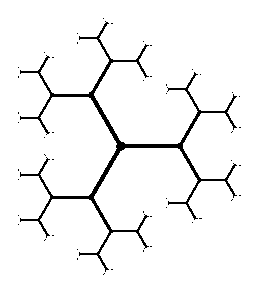
\includegraphics{covering-game.1.eps}

Picture 1

~

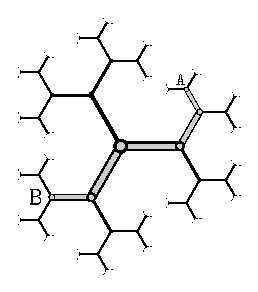
\includegraphics{covering-game.2.eps}

Picture 2

~

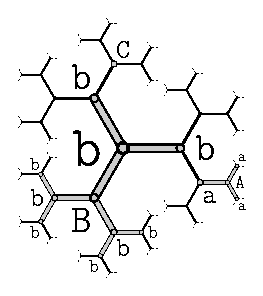
\includegraphics{covering-game.3.eps}

Picture 3

~

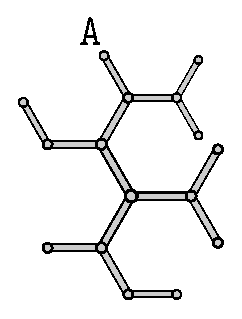
\includegraphics{covering-game.4.eps}

Picture 4

~


\includegraphics{covering-game.5.eps}

Picture 5
\end{center}
\end{minipage}
\end{tabular}

\newpage

Alice, Bob and Carl play a game on a discrete trine.
Firstly, they choose the playing field: it is some segment
of the discrete trine.
The game ends when all points of the playing field are covered;
initially, all points are considered not covered.
The players make moves in turn:
Alice moves first, Bob moves second, and Carl moves third.
A move consists of choosing a point on the segment that is not yet covered.
After that, a circle centered at that point is constructed.
The radius of this circle is the maximal non-negative integer such that
all points of the circle belong to the playing field and are not yet covered.
Finally, all points of the circle are declared covered.
The player who can not make the next turn loses the game.

Picture 6 shows some positions in the game and possible moves
in these positions.
The selected point is marked by a capital letter, and other points
of the circle covered by the move are marked by respective lowercase letters.
The double-circled points are the points covered earlier in the game.
Remember that a player chooses the center of the circle, but after that,
the radius can not be chosen: it must be the maximal possible for this center
in the current game position.

\begin{center}
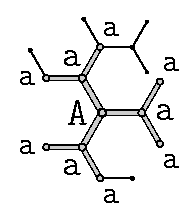
\includegraphics{covering-game.6.eps}
~~~~~
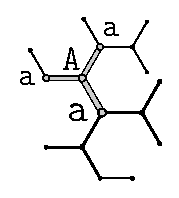
\includegraphics{covering-game.7.eps}
~~~~~
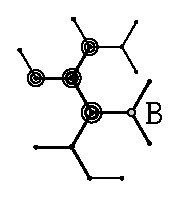
\includegraphics{covering-game.8.eps}
~~~~~
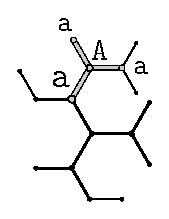
\includegraphics{covering-game.9.eps}
~~~~~
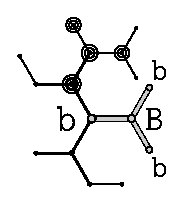
\includegraphics{covering-game.10.eps}

Picture 6
\end{center}

Who of the players can be forced to lose?
Player $X$ can be forced to lose if the other two players can team up
and act in such a way that $X$ will have no way not to lose the game.

\InputFile

The first line of input contains an integer $m$, the number of characters
in the string which specifies a left-hand traversal of the playing field.
The second line contains $m$ characters without spaces:
the left-hand traversal itself.
It is guaranteed that this traversal correctly specifies a segment
of a discrete trine, and this segment contains from $1$ to $100$ points.

\OutputFile

Print three lines.
On the first line, print whether it is possible to force Alice to lose,
on the second line, print the same for Bob, and on the third one, for Carl.
Each line should consist of the word ``\t{Yes}'' in case of positive answer
and ``\t{No}'' otherwise.

\Example

\begin{examplethree}
\exmp{%
6
llbrbb
}{%
No
Yes
No
}{%
\vskip 0pt

\includegraphics{covering-game.11.eps}
}%
\end{examplethree}

\Explanation

In this simple example, Alice has only two considerably different moves:
to choose one of the tree's leaves or the center vertex.

In the first case, only the chosen leaf will be covered, and each next move
will also cover only one point.
The total number of moves will be four.
When there will be no possible moves left, it will be Bob's turn.

In the second case, all points are covered on the first move.
Here, Bob also loses the game.

\end{problem}
